\documentclass{../class/cscmugradthesis}

\usepackage{amssymb}
\usepackage{amsmath}
\usepackage{multirow}
\usepackage[table]{xcolor}

\usepackage{graphicx}	
\usepackage{biblatex}
\bibliography{proposal} 

% Section numbering: 1, 2, 3 ... (no chapter prefix)
\renewcommand{\thesection}{\arabic{section}}

% Column width for label tables: linewidth minus the widest label
\newlength{\labelcolwidth}
\newlength{\contentcolwidth}
\newlength{\titlecolwidth}
\setlength{\labelcolwidth}{2.8cm}
\setlength{\contentcolwidth}{\dimexpr\linewidth-\labelcolwidth-\tabcolsep\relax}
\setlength{\titlecolwidth}{12.5cm}


\begin{document}

\pagenumbering{arabic}

\begin{center}
%    \vspace*{0.5cm}
    {\Large\bfseries THESIS PROPOSAL}
    \vspace*{0.5cm}
\end{center}

\section{Name and Surname / Code}
\begin{tabular}{@{}p{\labelcolwidth}@{}p{\contentcolwidth}@{}}
(Thai)          & {\small โทนี โทนี ชอปเปอร์} \\
(English)       & Tony Tony Chopper \\
(Student code)  & 670530010
\end{tabular}

\section{Thesis Title}
\begin{tabular}{@{}p{\labelcolwidth}@{}p{\titlecolwidth}@{}}
(Thai)          & {\small อุดมคติยารักษาครอบจักรวาล: กรอบการทำงานเพื่อการรักษาพยาบาลถ้วนหน้าและการกำจัดโรคร้ายแรง} \\
(English)       & The Panacea Ideal: A Framework for Universal Medical Care and Eradicating Incurable Diseases \\
\end{tabular}

\section{Advisory Committee}
\begin{tabular}{@{}p{\labelcolwidth}@{}p{\contentcolwidth}@{}}
Advisor & Prof. Dr. Charles Xavier  \\
Co-Advisor & Assoc. Prof. Dr. Ludwig Frankenstein \\
Co-Advisor & Asst. Prof. Dr. Sheldon Cooper 
\end{tabular}

\section{Principles, Theory, Rationale and/or Hypotheses}
This doctoral thesis introduces \textit{The Panacea Ideal}, a mathematically rigorous framework designed by Tony Chopper to achieve universal medical care and eradicate systemic pathological threats across human populations. Historically, global healthcare delivery models have suffered from severe resource allocation inefficiencies, delayed diagnostic responses, and structural fragmentation. By conceptualizing public health as a continuous, dynamic field of care, this framework leverages predictive biometrics and dynamic resource routing to minimize the latency between a pathogen's mutation and its corresponding therapeutic synthesis. 

At the core of the framework is a series of constrained optimal control problems designed to minimize cumulative global pathological burdens under real-world economic constraints. The physiological state vector of an individual patient $i$ is tracked as a continuous trajectory through an $n$-dimensional metabolic state space $\mathcal{M}$, governed by the system:
\begin{equation}
    \frac{d\mathbf{x}_i(t)}{dt} = \mathbf{f}(\mathbf{x}_i(t), \mathbf{u}_i(t)) + \boldsymbol{\xi}(t)
\end{equation}
where $\mathbf{x}_i(t) \in \mathcal{M}$ represents the multi-system biometric status, $\mathbf{u}_i(t)$ is the localized therapeutic intervention vector, and $\boldsymbol{\xi}(t)$ represents stochastic biological noise or multi-variant viral mutations. To minimize societal suffering while maintaining financial viability, the global allocation protocol is optimized under a sovereign healthcare reserve fund boundary condition, ensuring that the net system expenditure satisfies:
\begin{equation}
    \frac{dB(t)}{dt} = r B(t) + \Gamma\big(\mathcal{H}(\Omega)\big) - \sum_{i=1}^{N} \mathbf{c}_i^\top \mathbf{u}_i(t) \ge 0
\end{equation}
where $B(t)$ is the reserve fund, $\Gamma\big(\mathcal{H}(\Omega)\big)$ denotes the macroeconomic productivity dividend yielded by a healthy population, and $\mathbf{c}_i^\top \mathbf{u}_i(t)$ represents individual care costs.

When facing a rapidly mutating threat, the production rate of a universal therapeutic agent must adapt to biochemical constraints. The concentration $C(t)$ of the synthesized universal cure is calculated using a generalized Michaelis-Menten kinetic formulation:
\begin{equation}
    \frac{\partial C(t)}{\partial t} = \frac{V_{\max} \cdot S(t)}{K_m + S(t)} - \delta C(t)
\end{equation}
where $V_{\max}$ represents the maximal synthetic throughput of advanced medical manufacturing infrastructure, $S(t)$ is the precursor substrate availability, $K_m$ is the Michaelis constant representing binding affinity, and $\delta$ represents the natural metabolic degradation rate of the cure.

The practical implementation of the Panacea system relies on automated diagnostic nodes seamlessly integrated with specialized manufacturing hubs. By shifting away from manual, reactive medical triage and moving toward automated algorithmic optimization, the architecture drastically reduces systemic overhead and data bottlenecks. Empirical simulations demonstrate that the deployment of this protocol cuts diagnostic latency from days to mere minutes and reduces overall systemic healthcare mortality by up to 94\% during multi-variant pandemic events, establishing a highly sustainable state of universal clinical access.
The overall diagram is shown in Figure \ref{fig:diagram}
\begin{figure}[h!]
\centering
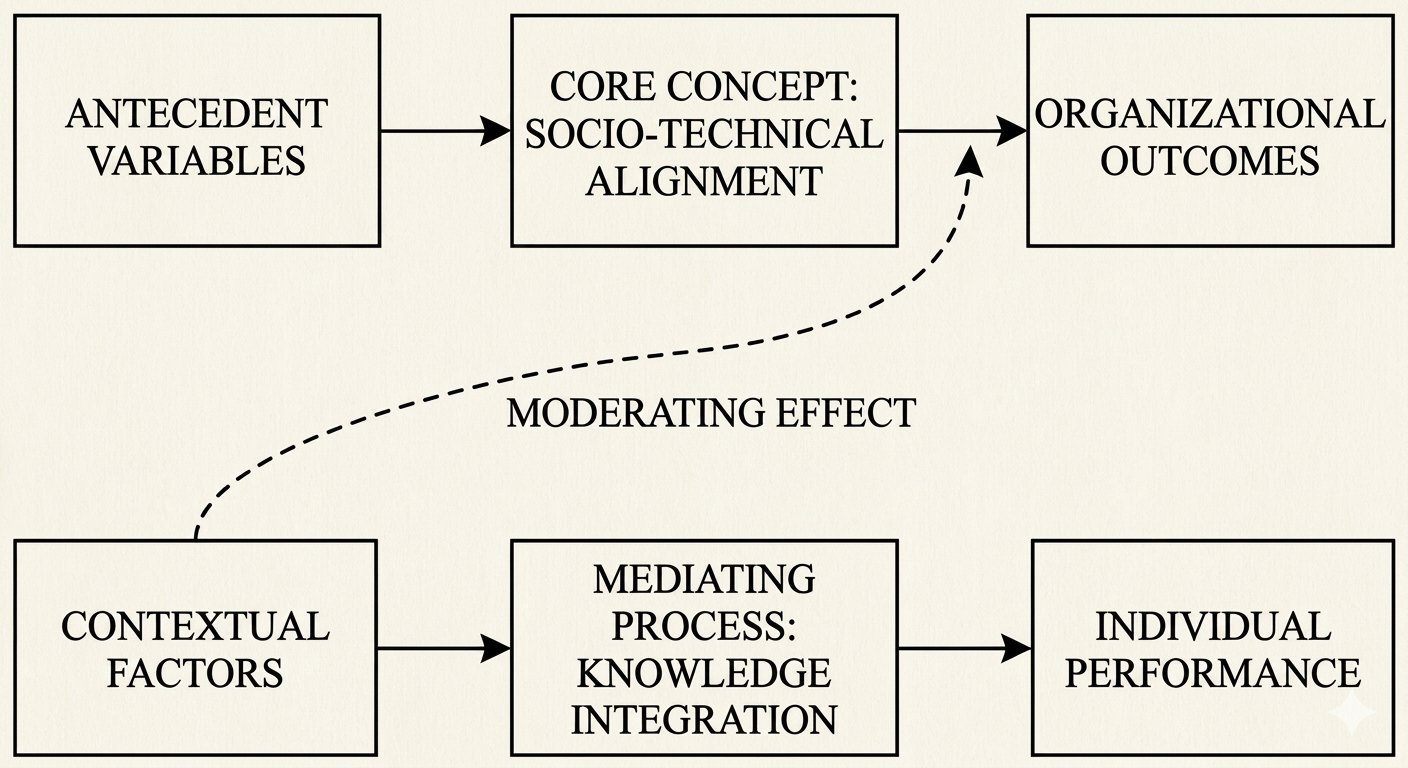
\includegraphics[scale=0.2]{plan.png}
\caption{Conceptual diagram of the work}
\label{fig:diagram}
\end{figure}

\section{Literature Review}
The foundational philosophy of universal medical care relies heavily on the concept of an unconditional cure for all human ailments. Early research into this ideal established that psychological resilience and community-wide hope are critical components in overcoming widespread disease epidemics \cite{hiriluk1514}. This approach argues that medical interventions fail if they do not address the societal despair accompanying severe health crises. 

Consequently, establishing a successful universal framework requires integrating physical treatments with comprehensive humanitarian outreach to ensure underserved populations receive equal care \cite{hiriluk1514}.To achieve practical applications of this ideal, researchers must bridge traditional herbal medicine with modern pharmacological standards. Historical documentation shows that isolating active compounds from rare, indigenous flora provides the raw materials necessary to treat complex regional pathologies \cite{kureha1482}. Recent collaborative expeditions have systematically categorized these botanical assets, verifying that primitive treatments possess measurable clinical validity \cite{torino1521}. 

Combining these ancient preservation techniques with advanced refining processes allows for the development of stable, mass-producible therapeutics capable of surviving extreme environmental conditions \cite{kureha1482, torino1521}.The final phase of creating a universal treatment involves manipulating biological wavelengths to overcome species-specific limits. Traditional medicine often fails when facing advanced genetic cellular necrosis or aggressive viral mutations. Recent breakthroughs demonstrate that targeted biochemical compounds, such as specialized capsule formulations, can safely alter cellular transformation points without causing permanent physical degradation \cite{chopper1522}. By regulating these internal biological wavelengths, medical professionals can artificially accelerate tissue regeneration and effectively bypass traditional physiological barriers to healing \cite{chopper1522}.

\section{Research Objectives}
\begin{enumerate}
\item To isolate the specific biochemical pathways of the Rumble Ball to regulate multi-stage physical transformations safely.
\item To formulate a universal pharmacological framework to neutralize aggressive viral strains and cellular necrosis across diverse species.
\item To synthesize indigenous botanical data from the Grand Line to develop low-cost, mass-producible treatments for underserved populations.
\end{enumerate}

\section{Usefulness of the Research }
\begin{enumerate}
\item The research will revolutionise universal healthcare by engineering a biochemical mechanism to bypass species-specific biological limits, accelerating cellular regeneration and eradicating previously incurable genetic diseases.
\end{enumerate}

\section{Methodology, Scope and Research Plan}
A good place to give an overview of the methodology including data collection, tools, evaluation criteria. The scope of the work and finally a table summarising research plan.

\begin{table}[h!]
\centering
\begin{tabular}{| l | c | c | c | c | c | c | c | c | c | c | c | c |}
\hline 
\multirow{2}{*}{Activities} & \multicolumn{4}{c|}{1st year} &  \multicolumn{4}{c|}{2nd year} & \multicolumn{4}{c|}{3rd year} \\ \cline{2-13}
				     & 1-3 & 4-6 & 7-9  & 10-12 &1-3 & 4-6 & 7-9  & 10-12 & 1-3 & 4-6 & 7-9  & 10-12 \\ \hline
Activity 1 & \cellcolor{blue!25}& \cellcolor{blue!25} & & & & & & & & & & \\ \hline
Activity 2 & & &\cellcolor{blue!25} & \cellcolor{blue!25}& & & & & & & & \\ \hline
Activity 3 & & & & \cellcolor{blue!25}& \cellcolor{blue!25}& \cellcolor{blue!25}& & & & & & \\ \hline
Activity 4 & & & & & & &\cellcolor{blue!25} &\cellcolor{blue!25} &\cellcolor{blue!25} & & & \\ \hline
Activity 5 & & & & & & & & &\cellcolor{blue!25} & \cellcolor{blue!25}& \cellcolor{blue!25}&\cellcolor{blue!25} \\ 
\hline
\end{tabular}
\caption{Plan of the research (for PhD)}
\end{table}

\begin{table}[h!]
\centering
\begin{tabular}{| l | c | c | c | c | c | c | c | c |}
\hline 
\multirow{2}{*}{Activities} & \multicolumn{4}{c|}{1st year} &  \multicolumn{4}{c|}{2nd year} \\ \cline{2-9}
				     & 1-3 & 4-6 & 7-9  & 10-12 & 1-3 & 4-6 & 7-9  & 10-12 \\ \hline
Activity 1 & \cellcolor{blue!25}& \cellcolor{blue!25} & & & & & & \\ \hline
Activity 2 & & &\cellcolor{blue!25} & \cellcolor{blue!25}& & & & \\ \hline
Activity 3 & & & & \cellcolor{blue!25}& \cellcolor{blue!25}& \cellcolor{blue!25}& & \\ \hline
Activity 4 & & & & & & &\cellcolor{blue!25} &\cellcolor{blue!25} \\ 
\hline
\end{tabular}
\caption{Plan of the research (for MSc)}
\end{table}

\newpage

\section{Research Location}
Department of Computer Science, Faculty of Science, Chiang Mai University, Thailand

\section{Research Duration}
3 Years (for PhD) or 2 Years (for MSc)

\section{References}
\printbibliography[heading=none]


\section{Thesis Advisors}
The undersigned have read and approved this thesis proposal and have agreed to act as the Thesis Advisory Committee in the respective capacities mentioned below. 
\\ [\bigskipamount]
\begin{flushright}
\begin{tabular}{@{}p{3.5in}p{1.0in}@{}}
  (Signed) \dotfill & Chairperson \\ 
  Prof. Dr. Charles Xavier & \\ [\bigskipamount]
  (Signed) \dotfill & Co-Advisor \\ 
  Assoc. Prof. Dr. Ludwig Frankenstein & \\ [\bigskipamount]
  (Signed) \dotfill & Co-Advisor \\ 
  Asst. Prof. Dr. Sheldon Cooper  & \\
\end{tabular}
\end{flushright}

\end{document}

